\section*{Problem Statement}
We aim to compute the numerical solution of the non-linear second-order ordinary differential equation
\[
    m \frac{d^2x}{dt^2} = -kx - lx^3 - b\frac{dx}{dt} + F_0 \cos(\omega t),
\]
where $k, l, b > 0$ and $F_0, \omega$ are constants. This equation describes a driven, damped, non-linear oscillator.

\section*{Methodology}
The given equation cannot be solved in closed form due to the cubic nonlinearity. A numerical scheme based on finite differences is applied to approximate the solution.

The update formula for the position is derived by discretizing time with step size $\Delta t$, leading to:
\[
    x_{n+1} = c_1 x_n + c_2 x_n^3 + c_3 x_{n-1} + c_4 \cos(\omega t_n),
\]
where the coefficients are functions of the parameters $m, k, l, b, F_0$, and $\Delta t$.

\subsection*{Pseudo-code}
\begin{enumerate}
    \item Initialize parameters: $m, k, l, b, F_0, \omega, \Delta t, t_{\max}$.
    \item Initialize solution:
    \[
        x(0) = x_0, \quad x(\Delta t) = x_0 + v_0 \Delta t.
    \]
    \item Compute coefficients $c, c_1, c_2, c_3, c_4$ from system parameters.
    \item For $n = 2,3,\dots,N$:
    \[
        x_{n+1} = c_1 x_n + c_2 x_n^3 + c_3 x_{n-1} + c_4 \cos(\omega t_n).
    \]
    \item Plot $x(t)$ versus $t$.
\end{enumerate}

\section*{Results}
The numerical simulation yields a time-domain trajectory of the oscillator. The solution exhibits oscillatory behavior with nonlinear distortion due to the cubic restoring force, damping, and external driving force.

\begin{figure}[h!]
    \centering
    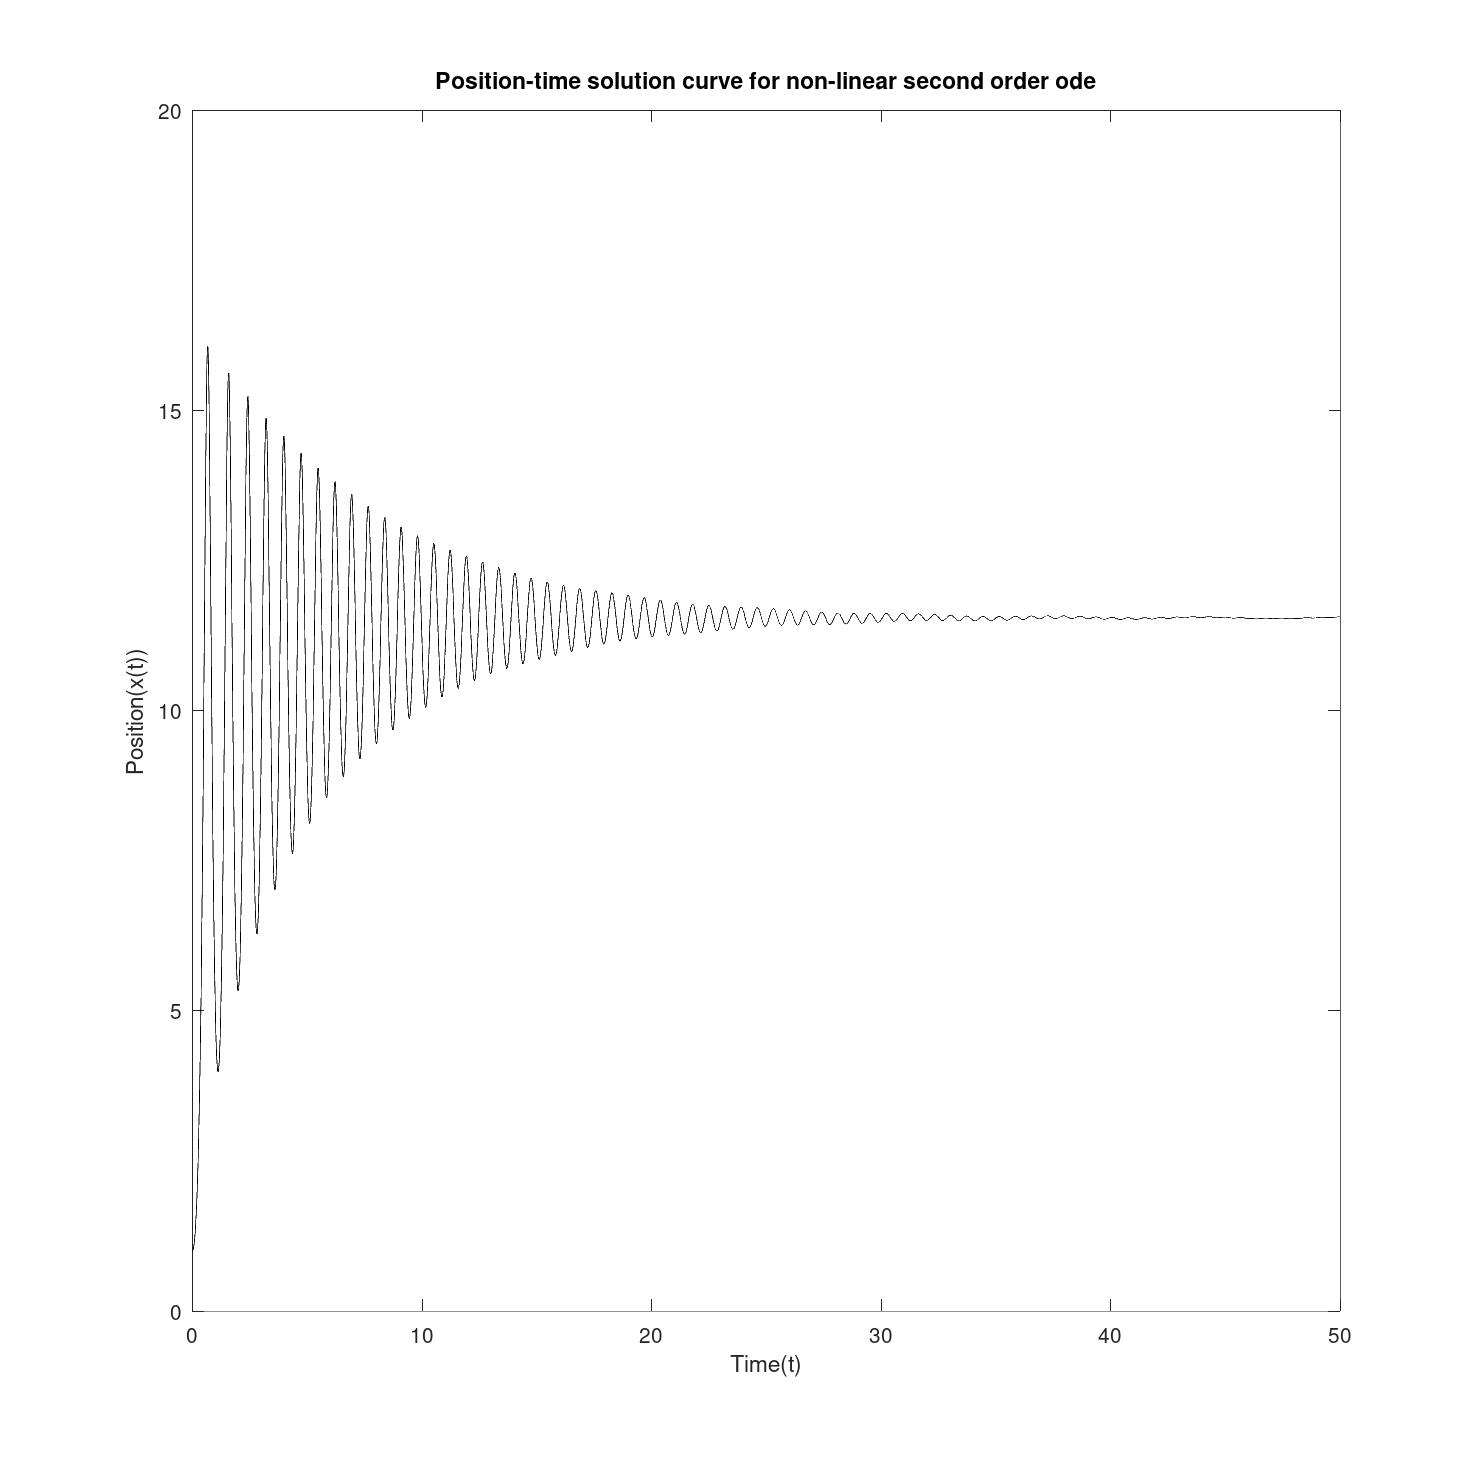
\includegraphics[width=0.85\textwidth]{a4.jpg}
    \caption{Position-time solution curve for the non-linear second-order ODE.}
\end{figure}

\section*{Conclusion}
The non-linear oscillator demonstrates rich dynamics that cannot be captured analytically. Numerical integration allows us to visualize the system's trajectory and analyze the influence of non-linearity, damping, and external driving. The results highlight the importance of computational methods in studying complex dynamical systems.
